\documentclass[a4paper]{article}
\usepackage{graphicx}
\title{\textbf{Dual Linear Regression Classification for Face Cluster Recognition}}
\date{}
\author{MANISH SHARMA - 2014A3PS181P\\Birla Institute of Technology and Science - Pilani \\ \texttt{f2014181@pilani.bits-pilani.ac.in}}

\begin{document}
	\maketitle
	\tableofcontents
	
	\section{Introduction}
	This project deals with the following face cluster recognition	problem: Given a galley set consists of a number of
	face image clusters, each containing the images of a known
	subject/identity; a probe cluster to be recognize contains
	a number of images of one subject; We are to match the
	probe cluster with the gallery set in order to determine the
	identity of the probe subject. The project is based on this paper.
	This should be taken to be
	a typical image set based face recognition problem and in this case it is LFW face database.
	
	\begin{figure}
		
			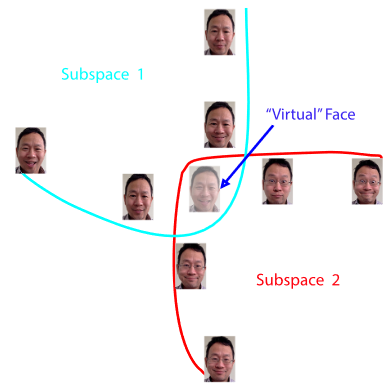
\includegraphics[scale=0.5]{fig1.png}
			\caption{ A "virtual" face in the intersection of two subspaces \label{fig1} }
		
		
	\end{figure}

	The simple but efficient linear regression based classifi-
	cation (LRC) approach was developed by Maseem, Togneri
	and Bennamoun. It gave the algorithm for face recognition using linear regression.

	Dual linear regression based
	classification (DLRC) algorithm generalizes the LRC ap-
	proach for the face cluster recognition problem. When com-
	paring two clusters of face images, we define the similarity
	between two clusters as the shortest distance between the
	subspaces each spanned from the face images of one cluster. In order to do so, DLRC attempts to find a “virtual” face
	image located in the intersection of the subspaces spanning
	from both clusters of downscaled face images (See Figure
	\ref{fig1}). The “distance” between the “virtual” face images recon-
	structed from both subspaces is then taken as the distance
	between these two subspaces. And the minimum distance found between the subspaces gives us the identity of the face.
	
	\section{State-of-the-art (Literature Survey)}
	Face recognition is a very important task in the fields of pattern recognition and computer vision because of its immense possible applications ranging from simple camera filters to needs in security. And their performance relies on the classifier used. A number of face recognition classifiers have been proposed. The most accurate ones are the following classifiers.
		\subsection{Face recognition classifiers}
		These classifiers use
		a single test sample for classification. Their classification
		performance, however, is generally dependent on the base
		or representation of individual test samples. 
		\subsubsection{Linear Regression Classifier (LRC)}
			In this proposed classifier it is assumed that samples from a specific object class are known to
			lie on a linear subspace. This concept is used to develop
			class-specific models of the registered users simply using the
			downsampled gallery images, thereby defining the task of face
			recognition as a problem of linear regression. 
			
			Least-squares
			estimation is used to estimate the vectors of parameters for a
			given probe against all class models. Finally, the decision rules in
			favor of the class with the most precise estimation. The proposed
			classifier can be categorized as a Nearest Subspace (NS) approach.
			
		\subsection{Face Cluster Recognition classifiers}
		Recently, researchers
		paid more attention to the image-set(Face images cluster) based classification which is much more accurate than any Face recognition classifiers. They use multiple test samples of the same class to form a cluster and used in classification.
		\subsubsection{Dual Linear Regression Classifier (DLRC)}
			For face cluster classification tasks, dual linear regression classification
			(DLRC) was proposed as a non-parametric approach.
			It borrows the idea of LRC and extends LRC
			from the single-query-sample based method to the image set/cluster
			based method. DLRC has a demonstrated better performance
			than a few well-known methods. However, DLRC
			considers only the related class-subspace for classification.
			That is to say, it pays attention only to minimizing the distance
			between the query set and the related train set.
		\subsubsection{Pairwise Linear Regression Classifier (PLRC)}
		PLRC and DLRC both follow the idea of
		restructuring the virtual sample of two image set for classification,
		and use the metric of the test set and the related
		train set.
		
		However as an improved
		version of DLRC, PLRC introduces the new unrelated
		subspace to maximize the distance between the query
		set and the unrelated images set, and utilizes a new combined
		metric that integrates a related metric and a new unrelated
		metric for classification.
		
		\subsection{Tackling Curse of Dimensionality}
			Face recognition systems are known to be critically dependent on
			manifold learning methods. A gray-scale face image of an order
			a ${\times}$ b can be represented as an ab-dimensional vector in the original
			image space. 
			
			However, any attempt at recognition in such a high dimensional
			space is vulnerable to a variety of issues often referred
			to as the curse of dimensionality. Therefore, at the feature extraction
			stage, images are transformed to low-dimensional vectors in the
			face space using downsampling. The main objective is to find such a basis function for this
			transformation which could distinguishably represent faces in the
			face space.
	
	\section{Proposed Approach}
	
		\subsection{Preprocessing Dataset}
					Firstly a subset of the dataset is extracted of persons having more than 20 face images.
			Also the images in lfw-a database are of the size 250${\times}$250. This includes the face and the background. Since background adds noise to the data we crop the images to the size of 90 ${\times}$78.
			These two things are done in the program filer.m .
			
			Next, we partition the data. The first 10 images of each person are taken as training data and the last 10 images are used as train/probe set. This is done using the programs partition.m and partition\_test.m .
		\subsection{Applying DLRC Algorithm}
			The DLRC classifier is using the algorithm given in the paper. This classifier is then used to predict the test/probe dataset. The accuracy is found out by -
			\[ Accuracy = (Correct predicted classes / Total predicted classes)  \times 100\]
			
			This is all done in the program dlrc.m .
			
		\subsection{Changes done}
			Only two changes are done in this project.
			
			Firstly, Instead of using downscaled images of sizes 10 ${\times}$10, the cropped images were used directly of sizes 90${\times}$ 78. It was done because the accuracy obtained from the downscaled images was coming out very less (near to 25\%).
			
			Secondly there is a correction in the paper. The equation (9) -
			
			\[  r_{1} = \hat{X_{c}}\left[ \beta^{c}_{1} ... \beta^{c}_{N_{c}-1}  \right]^{T} + x^{c}_{N_{c}} \]
			\[  r_{2} = \hat{Z}\left[ \beta^{c}_{N_{c}} ... \beta^{c}_{N_{c}+n-2}  \right]^{T} + y_{n} \]
			
			These equations are incorrect as there should not be transpose of ${\beta}$. It is wrong because the order of ${\hat{X_{c}}}$ is q${\times}$9 where q is size of each image and the order of ${\left[ \beta^{c}_{1} ... \beta^{c}_{N_{c}-1}  \right]^{T}}$ is 1${\times}$9. And we cannot multiply two matrices of the order q${\times}$9 and 1${\times}$9.
			
			So the correct equation is -
			
			\[  r_{1} = \hat{X_{c}}\left[ \beta^{c}_{1} ... \beta^{c}_{N_{c}-1}  \right] + x^{c}_{N_{c}} \]				
			\[  r_{2} = \hat{Z}\left[ \beta^{c}_{N_{c}} ... \beta^{c}_{N_{c}+n-2}  \right]^{T} + y_{n} \]
			
			
	\section{Result}
	
		\subsection{Database}
		For  DLRC, the database used for performance tests was LFW face database.
		
		LFW face database were captured in unconstrained environments
		such that there will be large variations in face images
		including pose,age, race, facial expression, lighting,
		occlusions, and background, etc. We use the aligned version
		of the LFW database, LFW-a database, to study the
		performance of the proposed classifiers. 
		
		All the
		images in LFW-a database are a size of 250 ${\times}$ 250. And for concentrating just on the faces and not the background, the images were cropped into
		a size of 90 ${\times}$78. A subset of LFW contains 62 persons,
		each people has more than 20 face images, is used for
		evaluating the algorithms. And in that, 10 images of each subject
		are selected to form the training set, while the last 10 image
		are used as the probe images.
		
		\subsection{Evironment used for Implementation}
		
		The operating system used is Windows 8.1  and programming is done on the software - MATLAB R2014a. 
		
				
		
			
			
			\subsection{Evaluation Criteria}
			The testing is done by passing the 62 face clusters (each having 10 images of the same person) from the test/probe set one by one to the DLRC classifier. And the predicted class is compared with the actual class of that cluster.
			
			\subsection{Observations}
			
			\begin{itemize}
				\item Correct predictions = 	58
				
				\item Total predictions		= 	62
				
				\item Accuracy of the DLRC classifier	=	93.55\%
			\end{itemize}
	
	\section{Conclusion}
						
			The Dual Linear Regression based Classifier (DLRC) for Facecluster Recognition MATLAB program was able to achieve the benchmark accuracy range given in the paper. The benchmark accuracy was in the range of 91.94\% to 95.16\% depending on the downscaled image size used. And the prediction accuracy of my program was 93.55%.
			
				
	
	
\end{document}